\documentclass[9pt,twocolumn,a4paper]{scrartcl}

\usepackage{lmodern}
\usepackage[top=19mm,bottom=19mm,left=14.32mm,right=14.32mm]{geometry}
\usepackage{graphicx}
\usepackage[font={small,it}]{caption}
\usepackage{hyperref}
\usepackage{titling}
\usepackage{amsmath}

\setlength{\droptitle}{-4em}

\usepackage{acronym}
\acrodef{IR}{Intermediate Representation}

\title{Code Transformation and Optimization Project, A.~Y.~2013-2014}
\def\realauthor{Marcello Pogliani}
\author{\realauthor \\[.3em]
        {\normalsize\itshape marcello.pogliani@mail.polimi.it}}

\makeatletter
\hypersetup{
    pdftitle={\@title},
    pdfauthor={\realauthor}
}
\makeatother

\begin{document}

\maketitle
\thispagestyle{empty}
\pagestyle{empty}

The project developed for the Code Transformation and Optimization course is a
set of LLVM intraprocedural passes aimed at converting C functions from a
floating point to a fixed point representation.
The target fixed-poin representation is two's complement 64-bit fixed point,
and the number of bits for the integer and decimal part is chosen by the
algorithm and may be different for each function of the same compilation unit.
The passes do not modify the return type of the function (the return value is
converted back to floating point).
Figure \ref{fig:project} reports the overall schema of the project.

\section{Design notes}

\paragraph{C source annotations} To enable the range analysis, the value range
of the function inputs should be known at compile time.
For this purpose, the C functions to be converted must contain an annotation
specifying the range of their parameters.
The initial ranges are expressed as a pair of integers (unsigned longs).
As an example, this snippet specifies that the variable \emph{param} can range
from $-10$ to $+10$:
\begin{verbatim}
double f(double param
         __attribute__((float_range(-10, 10))))
{
    /* body ... */
}
\end{verbatim}
The attribute is expressed in the LLVM \ac{IR} as a call to the intrinsic
\verb|llvm.float.range|. This intrinsic is not converted to any machine code,
but used by the analysis passes to retrieve the range information.

\paragraph{Range analysis} The \verb|float-range-analysis| pass retrieves the
initial range information from \verb|llvm.float.range| intrinsics and
forward-propagates it across the function.
For each supported floating point operation, it propagates the range of the
operands to the range of the result value according to the following rules:
\begin{align*}
&[a, b] + [c, d] = \left[a + b, c + d\right] \\
&[a, b] - [c, d] = \left[\min\{a - c, b - d\}, \max\{a - c, b - d\}\right] \\
&[a, b] \cdot [c, d] = \left[\min\{ac, bc, ad, bc\}, \max\{ac, bc, ad, bc\}\right] \\
&\frac{[a, b]}{[c, d]} = \left[\min\left\{\frac{a}{c}, \frac{b}{c}, \frac{a}{d}, \frac{b}{d}\right\},
                               \max\left\{\frac{a}{c}, \frac{b}{c}, \frac{a}{d}, \frac{b}{d}\right\}\right] \\
&\phi([a_1, b_1], \dots,  [a_n, b_n]) = \left[\min\{a_1, \dots, a_n\}, \max\{b_1, \dots, b_n\}\right]
\end{align*}
Every propagation operation with an operand having unbounded
(\verb|Range::Top|) range yields an unbounded result.

For a value having range $[x, y]$, the minimum number of bits required to store
the the integer part without overflow is
    \[ \left \lceil \log_2{\max(\tilde{x}, \tilde{y})} \right \rceil + 1\]
where $\tilde{x} = x + 1$ if $x \geq 0$ and $\tilde{x} = |x|$ if $x < 0$.
Globally, the minimum bit-width $IBW$ required to store the integer part of
each value is the maximum over the minimum integer bit-width of each value.

\begin{figure}
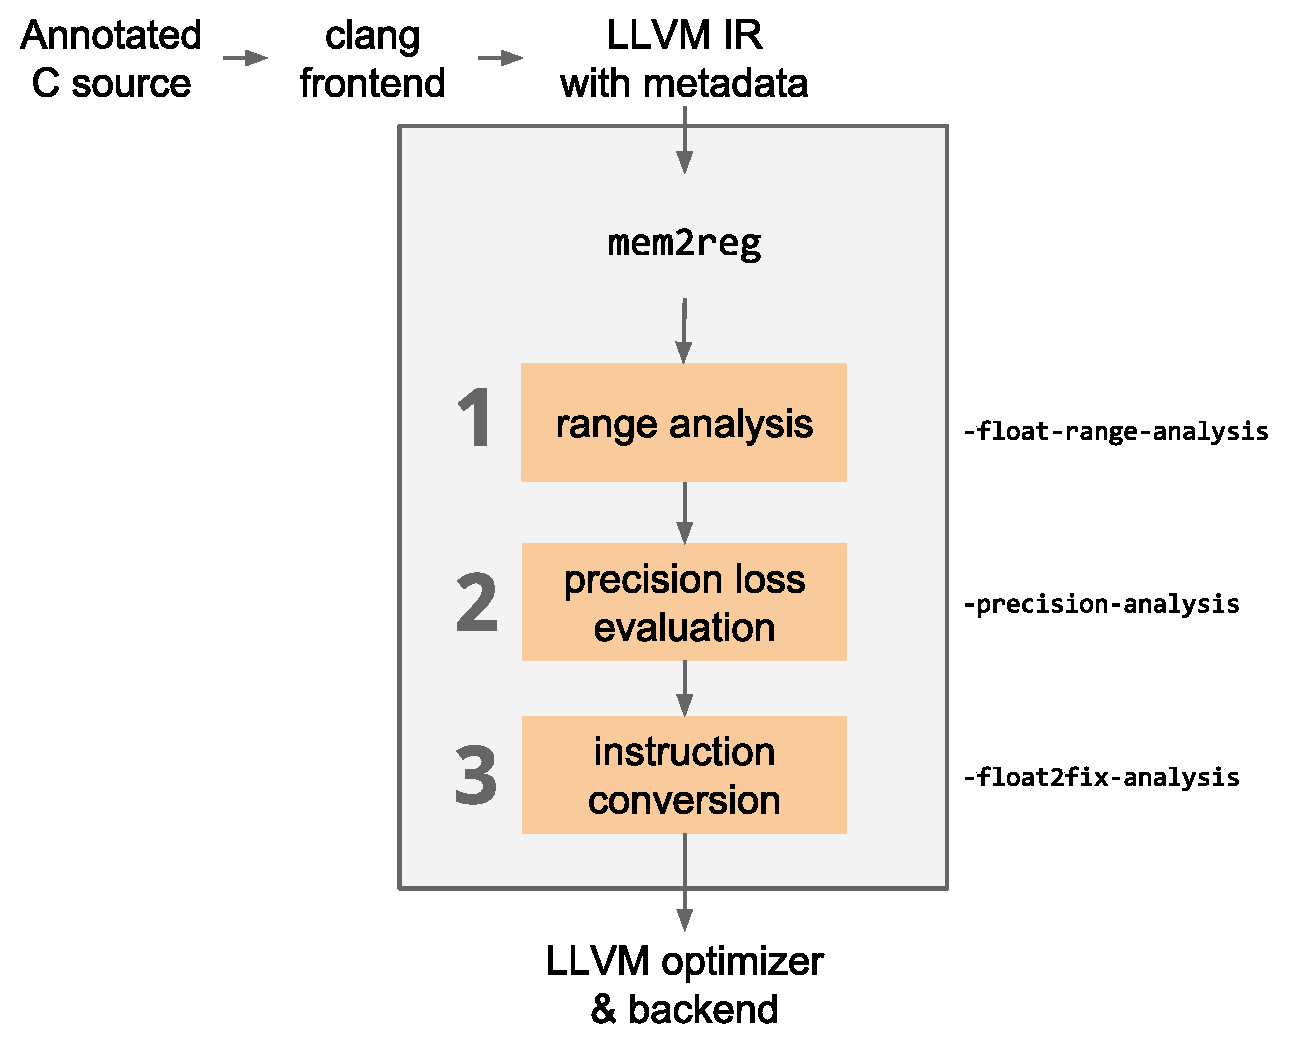
\includegraphics[width=\linewidth]{schema}
\caption{Project structure}\label{fig:project}
\end{figure}

\paragraph{Precision analysis} The \verb|precision-analysis| pass builds on the
results of the float range analysis to estimate the loss of precision due to
the conversion to a fixed point representation.

Let $IBW$ be the (minimum) number of bits for the integer part that avoids
overflow (computed by the previous pass); for our target representation the
number of bits $DBW$ for the decimal part are computed as:
    \[ DBW = \left\lfloor (64 - IBW) / 2 \right\rfloor \]
The most significant $DBW$ bits are unused -- this avoids to lose the most
significant bits of the operands during some operations (multiplication and
division).

The quantization (truncation) error due to the conversion from a floating point
representation to a fixed point one is estimated as $2^{-DBW}$. The pass
computes the loss of precision $err(\cdot)$ according to the following rules:
\begin{align*}
    err(a + b) &= err(a) + err(b) \\
    err(a - b) &= err(a) + err(b) \\
    err(a \cdot b) &= \max(|a|) \cdot err(b) + \max(|b|) \cdot err(a) + \\
               &  + err(a) \cdot err(b) + 2^{-DBW} \\
    err\left(\frac{a}{b}\right) &= \frac{\max(|a|)}{\max(b)^2} \cdot err(b)
                         + \frac{1}{\max(|b|)} \cdot err(a) + 2^{-DBW}
\end{align*}
where $\max(\cdot)$ is the maximum absolute value of the value, computed from
its range.

As a measure of the precision of the fixed point conversion, the pass uses the
``equivalent'' decimal bitwidths, i.e., the number of decimal bits so that the
error occurring in the fixed point version of the functions is not greater than
the quantization error when converting the floating point result to a fixed
point representation using that decimal bit-width.

\paragraph{Conversion} The conversion stage is implemented by the
\verb|float2fix| pass.

The pass supports the case where only some of the floating point instructions
in a given function should be transformed to fixed point.

For each instruction that can be converted (and for its operands), the pass
generates code to convert the floating point value into a fixed point one, and
inserts those instructions immediately after the \emph{definition} of the
value. Pointers to converted instructions are inserted into a data structure
for caching purposes. Then, the pass loops again on all the instructions, and
checks whether the parameters of any non-converted instructions have been
converted to fixed point. If this is the case, the pass creates a floating
point version after the definition of the fixed point version.

To convert a value $v$ to fixed point, the pass inserts a \verb|fmul|
instruction to compute $v \cdot 2^{DBW}$, followed by a cast to a 64 bit
integer; the reverse happens to convert the value back to floating point.

Operations are implemented as the corresponding integer operations on signed
64-bit integers; in the case of multiplication, the operation is followed by a
right shift (with sign extension) of $DBW$ bits; a left shift of $DBW$ bits is
inserted before the divisions to avoid losing the decimal part during the
operation.

The \verb|float2fix| pass does not remove the original floating point
instructions: the user is expected to run dead code elimination (\verb|-dce|)
afterwards.

\paragraph{Command line arguments} The pass recognizes the following arguments:
\begin{itemize}
\item \verb|precision-bitwidth| threshold to enable the conversion of a
function, in terms of the minimum number of equivalent decimal bit-width as
computed by the \verb|precision-analysis| pass;
\item \verb|internal-bitwidth| overrides the result of the precision analysis
pass and converts to fixed point all the instructions that are guaranteed not
to overflow using the number of bits for the decimal part specified at command
line, regardless of the precision loss.
\end{itemize}

\paragraph{Limitations}
\begin{itemize}
\item Both the range analysis and the precision analysis
perform propagation only in the case of simple loops where the trip-count can
be computed statically at compile-time; furthermore, propagation occurs
applying the transfer functions for the (statically known) number of loop
iterations, thus in case of a large trip count the passes may be fairly
inefficient; for loops with unknown trip-counts, an unbounded range is
considered.
\item During the range analysis, control dependencies are partly considered. When
propagating the value range to an instruction $i$, the pass checks whether $i$
is control dependent with respect to some condition concerning the operands of
$i$. If this is the case, the ranges of the operands used for the propagation
to the result of $i$ are constrained according to the condition, in a way
similar to the idea of \emph{range refinement function} propsed in
\cite{stephenson-2000-pldi}. Despite this, the pass fails at considering some
control-dependencies, especially in the \emph{else} branch of \emph{if}
statements: complex conditionals (e.g., \emph{if($x < 10.0$ \&\& $y > 4.0$)}) are
translated into the \ac{IR} as multiple branches, thus the basic block for the
\emph{else} branch can have multiple predecessors, making it difficult for the
algorithm to recognize the constraints.
\item The precision analysis step may benefit from the use of affine arithmetic to
propagate errors, as proposed in \cite{lee-2006-tcad,fanc-2003-iccad}.
\end{itemize}

\section{How to compile the source code}

The project requires to patch LLVM and clang with the implementation of the
\verb|llvm.float.range| intrinsics.

The project was developed and tested with LLVM 3.4 under Linux (in particular,
it is known to work with CentOS 6.x using clang 3.4 compiled from sources using
the stock gcc 4.4.x from the repositories).

The following instructions assume that
\begin{itemize}
\item \verb|LLVM_SRC| is the directory where the llvm source code is located
\item \verb|LLVM_BUILD| is the llvm build directory (separated from the source tree)
\end{itemize}
Download LLVM 3.4 and clang:
{\small
\begin{verbatim}
 $ wget http://llvm.org/releases/3.4/llvm-3.4.src.tar.gz
 $ tar xvf llvm-3.4.src.tar.gz
 $ mv llvm-3.4 $LLVM_SRC
 $ rm llvm-3.4.src.tar.gz
 $ cd $LLVM_SRC
 $ wget http://llvm.org/releases/3.4/clang-3.4.src.tar.gz
 $ tar xvf clang-3.4.src.tar.gz
 $ mv clang-3.4 tools/clang
 $ rm clang-3.4.src.tar.gz
\end{verbatim}
}
\noindent Move the directory with the project source code to \verb|projects/|:
{\small
\begin{verbatim}
 $ mv /where/float-range/is/ $LLVM_SRC/projects/float-range
\end{verbatim}
}
\noindent Apply the provided patch:
{\small
\begin{verbatim}
 $ cd $LLVM_SRC
 $ patch -p1 < projects/float-range/llvm-float-range.patch
 $ cd tools/clang
 $ patch -p1 < projects/float-range/clang-float-range.patch
\end{verbatim}
}
\noindent Configure LLVM, clang and the project in \verb|LLVM_BUILD|:
{\small
\begin{verbatim}
 $ mkdir -p $LLVM_BUILD
 $ cd $LLVM_BUILD
 $ $LLVM_SRC/configure
 $ mkdir -p $LLVM_BUILD/projects/float-range
 $ cd $LLVM_BUILD/projects/float-range
 $ $LLVM_SRC/projects/float-range/configure
\end{verbatim}
}
\noindent Finally, configure and compile it all:
{\small
\begin{verbatim}
 $ cd $LLVM_BUILD
 $ make
\end{verbatim}
}

\section{Usage example}
{\small
\begin{verbatim}
 $ ./clang -emit-llvm file.c -c -o in.bc
 $ ./opt -load /path/to/LLVMFloatRange.so -mem2reg -lcssa
         -float-range-analysis -precision-analysis -float2fix
         -dce -precision-bitwidth $PREC -S < in.bc > out.ll
\end{verbatim}


\nocite{*}
\bibliographystyle{plain}
\bibliography{references}
\end{document}
